\documentclass[a4paper, 11pt]{article}
\usepackage[utf8]{inputenc}
\usepackage[english]{babel}
\usepackage[utf8]{inputenc}
\usepackage[margin=3.cm]{geometry}
\usepackage{fancyhdr}

\usepackage[T1]{fontenc}
\usepackage{lmodern}

\usepackage{graphicx}
\graphicspath{ {images/} }
\usepackage{pdflscape}


\usepackage{array}

\usepackage{color,array}

\definecolor{mygray}{gray}{0.6} %custom color for text

\usepackage{float}
\usepackage[table,xcdraw]{xcolor}

\usepackage{multirow}
\usepackage{slashbox} % Defines \backslashbox{..}{..}
\usepackage{adjustbox}

\usepackage{varwidth} %for lists next to each other


%for circles
\usepackage{tikz}
\newcommand*\circled[1]{\tikz[baseline=(char.base)]{
            \node[shape=circle,draw,inner sep=2pt] (char) {#1};}}


%Includes "References" in the table of contents
\usepackage[nottoc]{tocbibind}

\usepackage{enumitem}
\setlist{nolistsep}

\fancypagestyle{plain}{%
  \renewcommand{\headrulewidth}{0pt}%
  \fancyhf{}%
  \fancyfoot[L]{\footnotesize Raymond Lochner}
  \fancyfoot[C]{\footnotesize October 2017 - Université libre de Bruxelles}%
  \fancyfoot[R]{\thepage}
}
\pagestyle{plain}

\date{\today}

\begin{document}

\begin{titlepage}
	\centering
	{\scshape\LARGE Université libre de Bruxelles \par}
	\vspace{1cm}
	{\scshape\Large INFO-F-409 - Learning Dynamics\par}
	\vspace{1.5cm}
	{\huge\bfseries {Assignment One\par}}
	\vspace{2cm}
	{\Large Raymond Lochner - 000443637\par}
	\vspace{0.5cm}
	{\Large raymond.lochner@ulb.ac.be}
	\vfill
	
	\setcounter{tocdepth}{2} %hides subsubsections in TOC
	\tableofcontents

\vfill
% Bottom of the page
	{\large \today \par}
\end{titlepage}

\newpage

\section{The Hawk-Dove game}

The Hawk-Dove game was first formulated by John Maynard Smith and Georg Prince in 1973 \cite{MaynardSmith1973}. The aim of the game is to gain a better understanding of conflicts in the animal kingdom. It consits of two players \{Player One, Player Two\} who have each two actions \{Hawk, Dove\}.The resulting payoff matrix can bee seen in Table \ref{tab-HawkDoveOriginal} where:
\begin{itemize}
  \item V = fitness value of winning resources in fight
  \item D = fitness costs of injury
  \item T = fitness costs of wasting time
\end{itemize}

and we assume that V,D,T $\geq$ 0.

\begin{table}[H]
\centering
\caption{Hawk-Dove Payoff Matrix}
\label{tab-HawkDoveOriginal}
\begin{tabular}{cl|ll|ll|}
\multicolumn{1}{l}{}                             &                       & \multicolumn{4}{c|}{Player Two}                                             \\ \cline{3-6} 
\multicolumn{1}{l}{}                             &                       & \multicolumn{2}{c|}{Hawk}              & \multicolumn{2}{c|}{Dove}          \\ \hline
\multicolumn{1}{c|}{\multirow{4}{*}{Player One}} & \multirow{2}{*}{Hawk} &         & \multicolumn{1}{r|}{(V-D)/2} &       & \multicolumn{1}{r|}{0}     \\
\multicolumn{1}{c|}{}                            &                       & (V-D)/2 &                              & V     &                            \\ \cline{2-6} 
\multicolumn{1}{c|}{}                            & \multirow{2}{*}{Dove} &         & \multicolumn{1}{r|}{V}       &       & \multicolumn{1}{r|}{V/2-T} \\
\multicolumn{1}{c|}{}                            &                       & 0       &                              & V/2-T &                            \\ \hline
\end{tabular}
\end{table}

In a mixed strategy game, we consider each player performing his action with a certain probability \textit{p} or \textit{q}, which results in the following payoff matrix displayed in Table \ref{tab-HawkDoveMixedStrategy}.

\begin{table}[H]
\centering
\caption{Hawk-Dove Probability Payoff Matrix}
\label{tab-HawkDoveMixedStrategy}
\begin{tabular}{cl|ll|ll|}
\multicolumn{1}{l}{}                             &                                & \multicolumn{4}{c|}{Player Two}                                             \\ \cline{3-6} 
\multicolumn{1}{l}{}                             &                                & \multicolumn{2}{c|}{P(Hawk)=q}         & \multicolumn{2}{c|}{P(Dove)=(1-q)} \\ \hline
\multicolumn{1}{c|}{\multirow{4}{*}{Player One}} & \multirow{2}{*}{P(Hawk)=p}     &         & \multicolumn{1}{r|}{(V-D)/2} &       & \multicolumn{1}{r|}{0}     \\
\multicolumn{1}{c|}{}                            &                                & (V-D)/2 &                              & V     &                            \\ \cline{2-6} 
\multicolumn{1}{c|}{}                            & \multirow{2}{*}{P(Dove)=(1-p)} &         & \multicolumn{1}{r|}{V}       &       & \multicolumn{1}{r|}{V/2-T} \\
\multicolumn{1}{c|}{}                            &                                & 0       &                              & V/2-T &                            \\ \hline
\end{tabular}
\end{table}

With this table we are able to calculate the payoff of the actions Hawk and Dove for Player One:

Player One's expected payoff for the strategy Hawk(p) is:
\[ q \times \frac{V-D}{2} + (1-q) \times V \]

Player One's expected payoff for the strategy Dove(1-p) is:
\[ q \times 0 + (1-q) \times ( \frac{V}{2} - T) = (1-q) \times ( \frac{V}{2} - T) \]

\hrule
\vspace{6pt}

The best response set is \{Hawk\} if:
\[ q \times \frac{V-D}{2} + (1-q) \times V < (1-q) \times ( \frac{V}{2} - T) \]

The best response set is \{Dove\} if:
\[ q \times \frac{V-D}{2} + (1-q) \times V > (1-q) \times ( \frac{V}{2} - T) \]

All the players mixed strategies are best responses if:
\[ q \times \frac{V-D}{2} + (1-q) \times V = (1-q) \times ( \frac{V}{2} - T) \]

As we are dealing with unknown variables, let's rewrite the equation for $q$:

\[ q \times \frac{V-D}{2} + (1-q) \times V = (1-q) \times ( \frac{V}{2} - T) \]

\[ \frac{qV}{2} - \frac{qD}{2} + V - qV = \frac{V}{2} - T - \frac{qV}{2} + qT \]

\[ - \frac{qD}{2} + V = \frac{V}{2} - T + qT \]

\[ \frac{V}{2} + T = \frac{qD}{2} + qT \]

\[ \frac{V}{2} + T = q( \frac{D}{2} + T) \]

\[ V + 2T = q( D + 2T) \]

\[ q = \frac{V + 2T}{D + 2T} \]

To find any pure or mixed strategy of this scenario, we have to look at different values for the variables V,D and T. In this case, we must respect the following constraints:

\[ 0\leq q\leq 1 \quad\mathrm{and}\quad 0 \leq \frac{V + 2T}{D + 2T} \leq 1 \quad\mathrm{and}\quad V,T,D \geq 0 \]

\subsection{T=0}

Let's start by considering the case where $T=0$. This leaves gives us the following options: 
\begin{itemize}[noitemsep]
  \item $V=0$ with $D=0$
  \item $V=0$ with $D>0$
  \item $V>0$ with $D=0$
  \item $V=D>0$
  \item $V>D>0$
  \item $D>V>0$
\end{itemize}

\subsubsection{T=0, V=0, D=0}

Any pure or mixed strategy is a best response. This yields the mixed strategy NE (Hawk,Dove) = $(p,1-p), p \in \{(0\leq p \leq 1) \}$.

\begin{table}[H]
\centering
\caption{V=T=0, D>0}
\begin{tabular}{cl|ll|ll|}
\multicolumn{1}{l}{}                             &                                & \multicolumn{4}{c|}{Player Two}                                                                 \\ \cline{3-6} 
\multicolumn{1}{l}{}                             &                                & \multicolumn{2}{c|}{P(Hawk)=q}                 & \multicolumn{2}{c|}{P(Dove)=(1-q)}             \\ \hline
\multicolumn{1}{c|}{\multirow{4}{*}{Player One}} & \multirow{2}{*}{P(Hawk)=p}     &             & \multicolumn{1}{r|}{\circled{0}} &             & \multicolumn{1}{r|}{\circled{0}} \\
\multicolumn{1}{c|}{}                            &                                & \circled{0} &                                  & \circled{0} &                                  \\ \cline{2-6} 
\multicolumn{1}{c|}{}                            & \multirow{2}{*}{P(Dove)=(1-p)} &             & \multicolumn{1}{r|}{\circled{0}} &             & \multicolumn{1}{r|}{\circled{0}} \\
\multicolumn{1}{c|}{}                            &                                & \circled{0} &                                  & \circled{0} &                                  \\ \hline
\end{tabular}
\end{table}

\subsubsection{T=0, V=0, D>0}

We have three pure strategy NE: \{Dove,Hawk\},\{Dove,Dove\} and \{Hawk,Dove\}. 

Player One's expected payoff for the strategy Hawk(p) is $- q \times \frac{D}{2}$.
Player One's expected payoff for the strategy Dove(1-p) is $0$. Solving for $q$ gives $q=0$ which does not yields a mixed strategy NE.

\begin{table}[H]
\centering
\caption{D>V=T=0}
\begin{tabular}{cl|ll|ll|}
\multicolumn{1}{l}{}                             &                                & \multicolumn{4}{c|}{Player Two}                                                                 \\ \cline{3-6} 
\multicolumn{1}{l}{}                             &                                & \multicolumn{2}{c|}{P(Hawk)=q}                 & \multicolumn{2}{c|}{P(Dove)=(1-q)}             \\ \hline
\multicolumn{1}{c|}{\multirow{4}{*}{Player One}} & \multirow{2}{*}{P(Hawk)=p}     &             & \multicolumn{1}{r|}{-D/2}        &             & \multicolumn{1}{r|}{\circled{0}} \\
\multicolumn{1}{c|}{}                            &                                & -D/2        &                                  & \circled{0} &                                  \\ \cline{2-6} 
\multicolumn{1}{c|}{}                            & \multirow{2}{*}{P(Dove)=(1-p)} &             & \multicolumn{1}{r|}{\circled{0}} &             & \multicolumn{1}{r|}{\circled{0}} \\
\multicolumn{1}{c|}{}                            &                                & \circled{0} &                                  & \circled{0} &                                  \\ \hline
\end{tabular}
\end{table}

\subsubsection{T=0, V>0, D=0}

We find the pure strategy NE \{Hawk,Hawk\}.

\begin{table}[H]
\centering
\caption{V>T=D=0}
\begin{tabular}{cl|ll|ll|}
\multicolumn{1}{l}{}                             &                                & \multicolumn{4}{c|}{Player Two}                                                             \\ \cline{3-6} 
\multicolumn{1}{l}{}                             &                                & \multicolumn{2}{c|}{P(Hawk)=q}                     & \multicolumn{2}{c|}{P(Dove)=(1-q)}     \\ \hline
\multicolumn{1}{c|}{\multirow{4}{*}{Player One}} & \multirow{2}{*}{P(Hawk)=p}     &               & \multicolumn{1}{r|}{\circled{V/2}} &             & \multicolumn{1}{r|}{0}   \\
\multicolumn{1}{c|}{}                            &                                & \circled{V/2} &                                    & \circled{V} &                          \\ \cline{2-6} 
\multicolumn{1}{c|}{}                            & \multirow{2}{*}{P(Dove)=(1-p)} &               & \multicolumn{1}{r|}{\circled{V}}   &             & \multicolumn{1}{r|}{V/2} \\
\multicolumn{1}{c|}{}                            &                                & 0             &                                    & V/2         &                          \\ \hline
\end{tabular}
\end{table}

\subsubsection{T=0, V=D>0}

We find the pure strategy NE's: \{Hawk,Hawk\}, \{Hawk,Dove\} and \{Dove,Hawk\}.

\begin{table}[H]
\centering
\caption{V=D>T=0}
\begin{tabular}{cl|ll|ll|}
\multicolumn{1}{l}{}                             &                                & \multicolumn{4}{c|}{Player Two}                                                                 \\ \cline{3-6} 
\multicolumn{1}{l}{}                             &                                & \multicolumn{2}{c|}{P(Hawk)=q}                 & \multicolumn{2}{c|}{P(Dove)=(1-q)}             \\ \hline
\multicolumn{1}{c|}{\multirow{4}{*}{Player One}} & \multirow{2}{*}{P(Hawk)=p}     &             & \multicolumn{1}{r|}{\circled{0}} &             & \multicolumn{1}{r|}{\circled{0}} \\
\multicolumn{1}{c|}{}                            &                                & \circled{0} &                                  & \circled{0} &                                  \\ \cline{2-6} 
\multicolumn{1}{c|}{}                            & \multirow{2}{*}{P(Dove)=(1-p)} &             & \multicolumn{1}{r|}{\circled{V}} &             & \multicolumn{1}{r|}{V/2}         \\
\multicolumn{1}{c|}{}                            &                                & \circled{0} &                                  & V/2         &                                  \\ \hline
\end{tabular}
\end{table}


\subsubsection{T=0, V>D>0}

The action \{Hawk, Hawk\} is always positive as we have $V>D$. We find the pure strategy NE \{Hawk,Hawk\}.

\begin{table}[H]
\centering
\caption{V>D>T=0}
\begin{tabular}{cl|ll|ll|}
\multicolumn{1}{l}{}                             &                                & \multicolumn{4}{c|}{Player Two}                                                                     \\ \cline{3-6} 
\multicolumn{1}{l}{}                             &                                & \multicolumn{2}{c|}{P(Hawk)=q}                             & \multicolumn{2}{c|}{P(Dove)=(1-q)}     \\ \hline
\multicolumn{1}{c|}{\multirow{4}{*}{Player One}} & \multirow{2}{*}{P(Hawk)=p}     &                   & \multicolumn{1}{r|}{\circled{(V-D)/2}} &             & \multicolumn{1}{r|}{0}   \\
\multicolumn{1}{c|}{}                            &                                & \circled{(V-D)/2} &                                        & \circled{V} &                          \\ \cline{2-6} 
\multicolumn{1}{c|}{}                            & \multirow{2}{*}{P(Dove)=(1-p)} &                   & \multicolumn{1}{r|}{\circled{V}}       &             & \multicolumn{1}{r|}{V/2} \\
\multicolumn{1}{c|}{}                            &                                & 0                 &                                        & V/2         &                          \\ \hline
\end{tabular}
\end{table}

\subsubsection{T=0, D>V>0}

The action \{Hawk, Hawk\} is always negative as we have $D>V$. We find two pure strategy NE's: \{Dove,Hawk\} and \{Hawk,Dove\}.

\begin{table}[H]
\centering
\caption{D>V>T=0}
\begin{tabular}{cl|ll|ll|}
\multicolumn{1}{l}{}                             &                                & \multicolumn{4}{c|}{Player Two}                                                                 \\ \cline{3-6} 
\multicolumn{1}{l}{}                             &                                & \multicolumn{2}{c|}{P(Hawk)=q}                 & \multicolumn{2}{c|}{P(Dove)=(1-q)}             \\ \hline
\multicolumn{1}{c|}{\multirow{4}{*}{Player One}} & \multirow{2}{*}{P(Hawk)=p}     &             & \multicolumn{1}{r|}{(V-D)/2}     &             & \multicolumn{1}{r|}{\circled{0}} \\
\multicolumn{1}{c|}{}                            &                                & (V-D)/2     &                                  & \circled{V} &                                  \\ \cline{2-6} 
\multicolumn{1}{c|}{}                            & \multirow{2}{*}{P(Dove)=(1-p)} &             & \multicolumn{1}{r|}{\circled{V}} &             & \multicolumn{1}{r|}{V/2}         \\
\multicolumn{1}{c|}{}                            &                                & \circled{0} &                                  & V/2         &                                  \\ \hline
\end{tabular}
\end{table}

Player One's expected payoff for the strategy Hawk(p) is:
\[ q \times \frac{V-D}{2} + (1-q) \times V = \frac{qV}{2} - \frac{qD}{2} + V - qV\]

Player One's expected payoff for the strategy Dove(1-p) is:
\[ q \times 0 + (1-q) \times V/2 = (1-q) \times (V/2) = \frac{V}{2} - \frac{qV}{2}\]

All the players mixed strategies are best responses if:
\[ \frac{qV}{2} - \frac{qD}{2} + V - qV = \frac{V}{2} - \frac{qV}{2} \]
\[ V - \frac{qD}{2} = \frac{V}{2} \]
\[ 2V - qD = V \]
\[ - qD = -V \]
\[q = \frac{V}{D} \]

We find the mixed strategy NE $q=\frac{V}{D}$. 

\subsection{V = 0}

Setting $V=0$ gives us the following options:
\begin{itemize}[noitemsep]
  \item $D=0$ with $T=0$ (already covered)
  \item $D=0$ with $T>0$
  \item $D>0$ with $T=0$ (already covered)
  \item $D=2T>0$
  \item $D>2T>0$
  \item $2T>D>0$
\end{itemize}

\subsubsection{V=0, D=0, T>0}

We find three pure strategy NE's: \{Hawk,Hawk\}, \{Hawk,Dove\} and \{Dove,Hawk\}.

\begin{table}[H]
\centering
\caption{T>V=D=0}
\begin{tabular}{cl|ll|ll|}
\multicolumn{1}{l}{}                             &                                & \multicolumn{4}{c|}{Player Two}                                                                 \\ \cline{3-6} 
\multicolumn{1}{l}{}                             &                                & \multicolumn{2}{c|}{P(Hawk)=q}                 & \multicolumn{2}{c|}{P(Dove)=(1-q)}             \\ \hline
\multicolumn{1}{c|}{\multirow{4}{*}{Player One}} & \multirow{2}{*}{P(Hawk)=p}     &             & \multicolumn{1}{r|}{\circled{0}} &             & \multicolumn{1}{r|}{\circled{0}} \\
\multicolumn{1}{c|}{}                            &                                & \circled{0} &                                  & \circled{0} &                                  \\ \cline{2-6} 
\multicolumn{1}{c|}{}                            & \multirow{2}{*}{P(Dove)=(1-p)} &             & \multicolumn{1}{r|}{\circled{0}} &             & \multicolumn{1}{r|}{-T}          \\
\multicolumn{1}{c|}{}                            &                                & \circled{0} &                                  & -T          &                                  \\ \hline
\end{tabular}
\end{table}

\subsubsection{V=0, D=2T>0}

Setting $D=2T$ gives the following payoff matrix:

\begin{table}[H]
\centering
\caption{D=2T>V=0}
\begin{tabular}{cl|ll|ll|}
\multicolumn{1}{l}{}                             &                                & \multicolumn{4}{c|}{Player Two}                                                                 \\ \cline{3-6} 
\multicolumn{1}{l}{}                             &                                & \multicolumn{2}{c|}{P(Hawk)=q}                 & \multicolumn{2}{c|}{P(Dove)=(1-q)}             \\ \hline
\multicolumn{1}{c|}{\multirow{4}{*}{Player One}} & \multirow{2}{*}{P(Hawk)=p}     &             & \multicolumn{1}{r|}{-T}          &             & \multicolumn{1}{r|}{\circled{0}} \\
\multicolumn{1}{c|}{}                            &                                & -T          &                                  & \circled{0} &                                  \\ \cline{2-6} 
\multicolumn{1}{c|}{}                            & \multirow{2}{*}{P(Dove)=(1-p)} &             & \multicolumn{1}{r|}{\circled{0}} &             & \multicolumn{1}{r|}{-T}          \\
\multicolumn{1}{c|}{}                            &                                & \circled{0} &                                  & -T          &                                  \\ \hline
\end{tabular}
\end{table}

We find two pure strategy NE's: \{Hawk,Dove\} and \{Dove,Hawk\}. Player One's expected payoff for the strategy Hawk(p) is: $-qT$. Player One's expected payoff for the strategy Dove(1-p) is: $-T + qT$. All the players mixed strategies are best responses if:
\[ -qT = -T + 2qT \]
\[ 2qT - T = 0 \]
\[ q = \frac{1}{2} \]

We find the mixed strategy NE: $q=\frac{1}{2}$. 

\subsubsection{V=0, D>2T>0}

We find two pure strategy NE's: \{Hawk,Dove\} and \{Dove,Hawk\}. Because $D>2T$, the action \{Hawk,Hawk\} is more negative than \{Dove,Dove\}.

\begin{table}[H]
\centering
\caption{D>2T>V=0}
\begin{tabular}{cl|ll|ll|}
\multicolumn{1}{l}{}                             &                                & \multicolumn{4}{c|}{Player Two}                                                                 \\ \cline{3-6} 
\multicolumn{1}{l}{}                             &                                & \multicolumn{2}{c|}{P(Hawk)=q}                 & \multicolumn{2}{c|}{P(Dove)=(1-q)}             \\ \hline
\multicolumn{1}{c|}{\multirow{4}{*}{Player One}} & \multirow{2}{*}{P(Hawk)=p}     &             & \multicolumn{1}{r|}{-D/2}        &             & \multicolumn{1}{r|}{\circled{0}} \\
\multicolumn{1}{c|}{}                            &                                & -D/2        &                                  & \circled{0} &                                  \\ \cline{2-6} 
\multicolumn{1}{c|}{}                            & \multirow{2}{*}{P(Dove)=(1-p)} &             & \multicolumn{1}{r|}{\circled{0}} &             & \multicolumn{1}{r|}{-T}          \\
\multicolumn{1}{c|}{}                            &                                & \circled{0} &                                  & -T          &                                  \\ \hline
\end{tabular}
\end{table}

Player One's expected payoff for the strategy Hawk(p) is: $-q\frac{D}{2}$. 

Player One's expected payoff for the strategy Dove(1-p) is: $-T + qT$. 

All the players mixed strategies are best responses if:
\[ -q\frac{D}{2} = -T + qT \]
\[ qT + \frac{qD}{2} = T \]
\[ 2qT + qD = 2T \]
\[ q(2T + D) = 2T \]
\[ q = \frac{2T}{2T + D} \]

We find the mixed strategy NE: $q = \frac{2T}{2T + D}$. 

\subsubsection{V=0, 2T>D>0}

Same pure and mixed strategy NE as previous section. The only difference here is that the action \{Dove,Dove\} is more negative than \{Hawk,Hawk\}.

\subsection{D = 0}

Setting $D=0$ gives us the following options:
\begin{itemize}[noitemsep]
  \setlength\itemsep{0.5em}
  \item $T=0$ with $V>0$ (already covered)
  \item $T>0$ with $V=0$ (already covered)
  \item $T=0$ with $V=0$ (already covered)
  \item $T=\frac{V}{2}>0$
  \item $T>\frac{V}{2} >0$
  \item $\frac{V}{2} > T>0$
\end{itemize}

\subsubsection{D=0, T=V/2>0}

We find the pure strategy NE \{Hawk,Hawk\}. 

\begin{table}[H]
\centering
\caption{T=V/2>D=0}
\begin{tabular}{cl|ll|ll|}
\multicolumn{1}{l}{}                             &                                & \multicolumn{4}{c|}{Player Two}                                                           \\ \cline{3-6} 
\multicolumn{1}{l}{}                             &                                & \multicolumn{2}{c|}{P(Hawk)=q}                     & \multicolumn{2}{c|}{P(Dove)=(1-q)}   \\ \hline
\multicolumn{1}{c|}{\multirow{4}{*}{Player One}} & \multirow{2}{*}{P(Hawk)=p}     &               & \multicolumn{1}{r|}{\circled{V/2}} &             & \multicolumn{1}{r|}{0} \\
\multicolumn{1}{c|}{}                            &                                & \circled{V/2} &                                    & \circled{V} &                        \\ \cline{2-6} 
\multicolumn{1}{c|}{}                            & \multirow{2}{*}{P(Dove)=(1-p)} &               & \multicolumn{1}{r|}{\circled{V}}   &             & \multicolumn{1}{r|}{0} \\
\multicolumn{1}{c|}{}                            &                                & 0             &                                    & 0           &                        \\ \hline
\end{tabular}
\end{table}

\subsubsection{D=0, T>V/2>0}

We find the pure strategy NE \{Hawk,Hawk\}. The action \{Dove,Dove\} is always negative.

\begin{table}[H]
\centering
\caption{T>V/2>D=0}
\begin{tabular}{cl|ll|ll|}
\multicolumn{1}{l}{}                             &                                & \multicolumn{4}{c|}{Player Two}                                                               \\ \cline{3-6} 
\multicolumn{1}{l}{}                             &                                & \multicolumn{2}{c|}{P(Hawk)=q}                     & \multicolumn{2}{c|}{P(Dove)=(1-q)}       \\ \hline
\multicolumn{1}{c|}{\multirow{4}{*}{Player One}} & \multirow{2}{*}{P(Hawk)=p}     &               & \multicolumn{1}{r|}{\circled{V/2}} &             & \multicolumn{1}{r|}{0}     \\
\multicolumn{1}{c|}{}                            &                                & \circled{V/2} &                                    & \circled{V} &                            \\ \cline{2-6} 
\multicolumn{1}{c|}{}                            & \multirow{2}{*}{P(Dove)=(1-p)} &               & \multicolumn{1}{r|}{\circled{V}}   &             & \multicolumn{1}{r|}{V/2-T} \\
\multicolumn{1}{c|}{}                            &                                & 0             &                                    & V/2-T       &                            \\ \hline
\end{tabular}
\end{table}

\subsubsection{D=0, V/2>T>0}

Same answer as previous configuration. Only difference is that the action \{Dove,Dove\} is always positive.

\subsection{T>0, V>0, D>0}

We can now look at configurations without a zero variable. This setting leaves us with the following configurations to consider:

\begin{varwidth}[t]{.33\textwidth}
T largest :
\begin{itemize}
  \setlength\itemsep{0.5em}
  \item $T=\frac{V}{2}=\frac{D}{2}$
  \item $T=\frac{V}{2}>\frac{D}{2}$
  \item $T=\frac{D}{2}>\frac{V}{2}$
  \item $T>\frac{V}{2}=\frac{D}{2}$
  \item $T>\frac{V}{2}>\frac{D}{2}$
  \item $T>\frac{D}{2}>\frac{V}{2}$
\end{itemize}
\end{varwidth}% <---- Don't forget this %
\hspace{4em}% <---- Don't forget this %
\begin{varwidth}[t]{.33\textwidth}
V/2 largest :
\begin{itemize}
  \setlength\itemsep{0.5em}
  \item \textcolor{mygray}{$\frac{V}{2}=\frac{D}{2}=T$} %already covered
  \item $\frac{V}{2}=\frac{D}{2}>T$
  \item \textcolor{mygray}{$\frac{V}{2}=T>\frac{D}{2}$} %already covered
  \item $\frac{V}{2}>\frac{D}{2}=T$
  \item $\frac{V}{2}>\frac{D}{2}>T$
  \item $\frac{V}{2}>T>\frac{D}{2}$
\end{itemize}
\end{varwidth}
\hspace{4em}% <---- Don't forget this %
\begin{varwidth}[t]{.33\textwidth}
D/2 largest :
\begin{itemize}
  \setlength\itemsep{0.5em}
  \item \textcolor{mygray}{$\frac{D}{2}=\frac{V}{2}=T$} %already covered
  \item \textcolor{mygray}{$\frac{D}{2}=\frac{V}{2}>T$}
  \item \textcolor{mygray}{$\frac{D}{2}=T > \frac{V}{2}$}
  \item $D/2>\frac{V}{2}=T$
  \item $D/2>\frac{V}{2}>T$
  \item $D/2>T>\frac{V}{2}$
\end{itemize}
\end{varwidth}


It should be noted that we only consider configurations around their extreme points, i.e. configurations that change the value of a cell(negative, zero or positive). Greyed out items are already considered by previous configurations.

\subsubsection{T=V/2=D/2}

We find three pure strategy NE's: \{Hawk,Hawk\}, \{Dove,Hawk\} and \{Hawk,Dove\}

\begin{table}[H]
\centering
\caption{T=V/2=D/2}
\begin{tabular}{cl|ll|ll|}
\multicolumn{1}{l}{}                             &                                & \multicolumn{4}{c|}{Player Two}                                                                 \\ \cline{3-6} 
\multicolumn{1}{l}{}                             &                                & \multicolumn{2}{c|}{P(Hawk)=q}                 & \multicolumn{2}{c|}{P(Dove)=(1-q)}             \\ \hline
\multicolumn{1}{c|}{\multirow{4}{*}{Player One}} & \multirow{2}{*}{P(Hawk)=p}     &             & \multicolumn{1}{r|}{\circled{0}} &             & \multicolumn{1}{r|}{\circled{0}} \\
\multicolumn{1}{c|}{}                            &                                & \circled{0} &                                  & \circled{V} &                                  \\ \cline{2-6} 
\multicolumn{1}{c|}{}                            & \multirow{2}{*}{P(Dove)=(1-p)} &             & \multicolumn{1}{r|}{\circled{V}} &             & \multicolumn{1}{r|}{0}           \\
\multicolumn{1}{c|}{}                            &                                & \circled{0} &                                  & 0           &                                  \\ \hline
\end{tabular}
\end{table}

\subsubsection{T=V/2>D/2}

We find the pure strategy NE: \{Hawk,Hawk\}.

\begin{table}[H]
\centering
\caption{T=V/2>D/2}
\begin{tabular}{cl|ll|ll|}
\multicolumn{1}{l}{}                             &                                & \multicolumn{4}{c|}{Player Two}                                                                   \\ \cline{3-6} 
\multicolumn{1}{l}{}                             &                                & \multicolumn{2}{c|}{P(Hawk)=q}                             & \multicolumn{2}{c|}{P(Dove)=(1-q)}   \\ \hline
\multicolumn{1}{c|}{\multirow{4}{*}{Player One}} & \multirow{2}{*}{P(Hawk)=p}     &                   & \multicolumn{1}{r|}{\circled{(V-D)/2}} &             & \multicolumn{1}{r|}{0} \\
\multicolumn{1}{c|}{}                            &                                & \circled{(V-D)/2} &                                        & \circled{V} &                        \\ \cline{2-6} 
\multicolumn{1}{c|}{}                            & \multirow{2}{*}{P(Dove)=(1-p)} &                   & \multicolumn{1}{r|}{\circled{V}}       &             & \multicolumn{1}{r|}{0} \\
\multicolumn{1}{c|}{}                            &                                & 0                 &                                        & 0           &                        \\ \hline
\end{tabular}
\end{table}


\subsubsection{T=D/2>V/2}

We find two pure strategy NE's: \{Hawk,Dove\} and \{Dove,Hawk\}. The actions \{Hawk,Hawk\} and \{Dove,Dove\} are always negative because $D>V$ and $T>V/2$.

\begin{table}[H]
\centering
\caption{T=D/2>V/2}
\begin{tabular}{cl|ll|ll|}
\multicolumn{1}{l}{}                             &                                & \multicolumn{4}{c|}{Player Two}                                                                 \\ \cline{3-6} 
\multicolumn{1}{l}{}                             &                                & \multicolumn{2}{c|}{P(Hawk)=q}                 & \multicolumn{2}{c|}{P(Dove)=(1-q)}             \\ \hline
\multicolumn{1}{c|}{\multirow{4}{*}{Player One}} & \multirow{2}{*}{P(Hawk)=p}     &             & \multicolumn{1}{r|}{(V-D)/2}     &             & \multicolumn{1}{r|}{\circled{0}} \\
\multicolumn{1}{c|}{}                            &                                & (V-D)/2     &                                  & \circled{V} &                                  \\ \cline{2-6} 
\multicolumn{1}{c|}{}                            & \multirow{2}{*}{P(Dove)=(1-p)} &             & \multicolumn{1}{r|}{\circled{V}} &             & \multicolumn{1}{r|}{V/2-T}       \\
\multicolumn{1}{c|}{}                            &                                & \circled{0} &                                  & V/2-T       &                                  \\ \hline
\end{tabular}
\end{table}

To find the mixed strategy NE, we need to calculate $q$ from the payoff matrix, which we already did earlier: $q = \frac{V + 2T}{D + 2T}$. 

\subsubsection{T>V/2=D/2}

We find three pure strategy NE's: \{Hawk,Hawk\}, \{Dove,Hawk\} and \{Hawk,Dove\}. The action \{Dove,Dove\} is always negative

\begin{table}[H]
\centering
\caption{T=V/2=D/2}
\begin{tabular}{cl|ll|ll|}
\multicolumn{1}{l}{}                             &                                & \multicolumn{4}{c|}{Player Two}                                                                 \\ \cline{3-6} 
\multicolumn{1}{l}{}                             &                                & \multicolumn{2}{c|}{P(Hawk)=q}                 & \multicolumn{2}{c|}{P(Dove)=(1-q)}             \\ \hline
\multicolumn{1}{c|}{\multirow{4}{*}{Player One}} & \multirow{2}{*}{P(Hawk)=p}     &             & \multicolumn{1}{r|}{\circled{0}} &             & \multicolumn{1}{r|}{\circled{0}} \\
\multicolumn{1}{c|}{}                            &                                & \circled{0} &                                  & \circled{V} &                                  \\ \cline{2-6} 
\multicolumn{1}{c|}{}                            & \multirow{2}{*}{P(Dove)=(1-p)} &             & \multicolumn{1}{r|}{\circled{V}} &             & \multicolumn{1}{r|}{V/2-T}       \\
\multicolumn{1}{c|}{}                            &                                & \circled{0} &                                  & V/2-T       &                                  \\ \hline
\end{tabular}
\end{table}

\subsubsection{T>V/2>D/2}

We find the pure strategy NE: \{Hawk,Hawk\}. The action \{Dove,Dove\} is always negative

\begin{table}[H]
\centering
\caption{T>V/2>D/2}
\begin{tabular}{cl|ll|ll|}
\multicolumn{1}{l}{}                             &                                & \multicolumn{4}{c|}{Player Two}                                                                       \\ \cline{3-6} 
\multicolumn{1}{l}{}                             &                                & \multicolumn{2}{c|}{P(Hawk)=q}                             & \multicolumn{2}{c|}{P(Dove)=(1-q)}       \\ \hline
\multicolumn{1}{c|}{\multirow{4}{*}{Player One}} & \multirow{2}{*}{P(Hawk)=p}     &                   & \multicolumn{1}{r|}{\circled{(V-D)/2}} &             & \multicolumn{1}{r|}{0}     \\
\multicolumn{1}{c|}{}                            &                                & \circled{(V-D)/2} &                                        & \circled{V} &                            \\ \cline{2-6} 
\multicolumn{1}{c|}{}                            & \multirow{2}{*}{P(Dove)=(1-p)} &                   & \multicolumn{1}{r|}{\circled{V}}       &             & \multicolumn{1}{r|}{V/2-T} \\
\multicolumn{1}{c|}{}                            &                                & 0                 &                                        & V/2-T       &                            \\ \hline
\end{tabular}
\end{table}

\subsubsection{T>D/2>V/2}

We find two pure strategy NE's: \{Hawk,Dove\} and \{Dove,Hawk\}. The actions \{Dove,Dove\} and \{Hawk,Hawk\} are always negative.

\begin{table}[H]
\centering
\caption{T>V/2>D/2}
\begin{tabular}{cl|ll|ll|}
\multicolumn{1}{l}{}                             &                                & \multicolumn{4}{c|}{Player Two}                                                                 \\ \cline{3-6} 
\multicolumn{1}{l}{}                             &                                & \multicolumn{2}{c|}{P(Hawk)=q}                 & \multicolumn{2}{c|}{P(Dove)=(1-q)}             \\ \hline
\multicolumn{1}{c|}{\multirow{4}{*}{Player One}} & \multirow{2}{*}{P(Hawk)=p}     &             & \multicolumn{1}{r|}{(V-D)/2}     &             & \multicolumn{1}{r|}{\circled{0}} \\
\multicolumn{1}{c|}{}                            &                                & (V-D)/2     &                                  & \circled{V} &                                  \\ \cline{2-6} 
\multicolumn{1}{c|}{}                            & \multirow{2}{*}{P(Dove)=(1-p)} &             & \multicolumn{1}{r|}{\circled{V}} &             & \multicolumn{1}{r|}{V/2-T}       \\
\multicolumn{1}{c|}{}                            &                                & \circled{0} &                                  & V/2-T       &                                  \\ \hline
\end{tabular}
\end{table}

To find the mixed strategy NE, we need to calculate $q$ from the payoff matrix, which we already did earlier: $q = \frac{V + 2T}{D + 2T}$. 

\vspace{6pt}
\hrule
\vspace{6pt}

\subsubsection{V/2=D/2>T}

We find three pure strategy NE's: \{Hawk,Hawk\}, \{Hawk,Dove\} and \{Dove,Hawk\}.

\begin{table}[H]
\centering
\caption{V/2=D/2>T}
\begin{tabular}{cl|ll|ll|}
\multicolumn{1}{l}{}                             &                                & \multicolumn{4}{c|}{Player Two}                                                                 \\ \cline{3-6} 
\multicolumn{1}{l}{}                             &                                & \multicolumn{2}{c|}{P(Hawk)=q}                 & \multicolumn{2}{c|}{P(Dove)=(1-q)}             \\ \hline
\multicolumn{1}{c|}{\multirow{4}{*}{Player One}} & \multirow{2}{*}{P(Hawk)=p}     &             & \multicolumn{1}{r|}{\circled{0}} &             & \multicolumn{1}{r|}{\circled{0}} \\
\multicolumn{1}{c|}{}                            &                                & \circled{0} &                                  & \circled{V} &                                  \\ \cline{2-6} 
\multicolumn{1}{c|}{}                            & \multirow{2}{*}{P(Dove)=(1-p)} &             & \multicolumn{1}{r|}{\circled{V}} &             & \multicolumn{1}{r|}{V/2-T}       \\
\multicolumn{1}{c|}{}                            &                                & \circled{0} &                                  & V/2-T       &                                  \\ \hline
\end{tabular}
\end{table}

\subsubsection{V/2>D/2=T}

We find the pure strategy NE: \{Hawk,Hawk\}.

\begin{table}[H]
\centering
\caption{V/2>D/2=T}
\begin{tabular}{cl|ll|ll|}
\multicolumn{1}{l}{}                             &                                & \multicolumn{4}{c|}{Player Two}                                                                       \\ \cline{3-6} 
\multicolumn{1}{l}{}                             &                                & \multicolumn{2}{c|}{P(Hawk)=q}                             & \multicolumn{2}{c|}{P(Dove)=(1-q)}       \\ \hline
\multicolumn{1}{c|}{\multirow{4}{*}{Player One}} & \multirow{2}{*}{P(Hawk)=p}     &                   & \multicolumn{1}{r|}{\circled{(V-D)/2}} &             & \multicolumn{1}{r|}{0}     \\
\multicolumn{1}{c|}{}                            &                                & \circled{(V-D)/2} &                                        & \circled{V} &                            \\ \cline{2-6} 
\multicolumn{1}{c|}{}                            & \multirow{2}{*}{P(Dove)=(1-p)} &                   & \multicolumn{1}{r|}{\circled{V}}       &             & \multicolumn{1}{r|}{V/2-T} \\
\multicolumn{1}{c|}{}                            &                                & 0                 &                                        & V/2-T       &                            \\ \hline
\end{tabular}
\end{table}

\subsubsection{V/2>D/2>T}

Same result as previous section.

\subsubsection{V/2>T>D/2}

Same result as previous section.

\vspace{6pt}
\hrule
\vspace{6pt}

\subsubsection{D/2>V/2=T}

We find two pure strategy NE's: \{Hawk,Dove\} and \{Dove,Hawk\}.

\begin{table}[H]
\centering
\caption{D/2>V/2=T}
\begin{tabular}{cl|ll|ll|}
\multicolumn{1}{l}{}                             &                                & \multicolumn{4}{c|}{Player Two}                                                                 \\ \cline{3-6} 
\multicolumn{1}{l}{}                             &                                & \multicolumn{2}{c|}{P(Hawk)=q}                 & \multicolumn{2}{c|}{P(Dove)=(1-q)}             \\ \hline
\multicolumn{1}{c|}{\multirow{4}{*}{Player One}} & \multirow{2}{*}{P(Hawk)=p}     &             & \multicolumn{1}{r|}{(V-D)/2}     &             & \multicolumn{1}{r|}{\circled{0}} \\
\multicolumn{1}{c|}{}                            &                                & (V-D)/2     &                                  & \circled{V} &                                  \\ \cline{2-6} 
\multicolumn{1}{c|}{}                            & \multirow{2}{*}{P(Dove)=(1-p)} &             & \multicolumn{1}{r|}{\circled{V}} &             & \multicolumn{1}{r|}{0}           \\
\multicolumn{1}{c|}{}                            &                                & \circled{0} &                                  & 0           &                                  \\ \hline
\end{tabular}
\end{table}

Player One's expected payoff for the strategy Hawk(p) is:
\[ q \times \frac{V-D}{2} + (1-q) \times V = -\frac{qV}{2} - \frac{qD}{2} + V\]

Player One's expected payoff for the strategy Dove(1-p) is:
\[ q\times 0 + (1-q) \times 0 = 0 \]

All the players mixed strategies are best responses if:
\[ -\frac{qV}{2} - \frac{qD}{2} + V = 0 \]
\[ qV + qD = 2V \]
\[ q(V + D) = 2V \]
\[ q = \frac{2V}{(V + D)} \]

We find a mixed strategy NE with $q=\frac{2V}{(V + D)}$.

\subsubsection{D/2>V/2>T}

We find two pure strategy NE's: \{Hawk,Dove\} and \{Dove,Hawk\}.

\begin{table}[H]
\centering
\caption{D/2>V/2=T}
\begin{tabular}{cl|ll|ll|}
\multicolumn{1}{l}{}                             &                                & \multicolumn{4}{c|}{Player Two}                                                                 \\ \cline{3-6} 
\multicolumn{1}{l}{}                             &                                & \multicolumn{2}{c|}{P(Hawk)=q}                 & \multicolumn{2}{c|}{P(Dove)=(1-q)}             \\ \hline
\multicolumn{1}{c|}{\multirow{4}{*}{Player One}} & \multirow{2}{*}{P(Hawk)=p}     &             & \multicolumn{1}{r|}{(V-D)/2}     &             & \multicolumn{1}{r|}{\circled{0}} \\
\multicolumn{1}{c|}{}                            &                                & (V-D)/2     &                                  & \circled{V} &                                  \\ \cline{2-6} 
\multicolumn{1}{c|}{}                            & \multirow{2}{*}{P(Dove)=(1-p)} &             & \multicolumn{1}{r|}{\circled{V}} &             & \multicolumn{1}{r|}{V/2-T}       \\
\multicolumn{1}{c|}{}                            &                                & \circled{0} &                                  & V/2-T       &                                  \\ \hline
\end{tabular}
\end{table}

To find the mixed strategy NE, we need to calculate $q$ from the payoff matrix, which we already did earlier: $q = \frac{V + 2T}{D + 2T}$. 

\subsubsection{D/2>T>V/2}

Same response as previous section.

\subsection{Results}

\subsubsection{Question 1}

The following are all the mixed strategy Nash equilibria (MSNE) of this game:
\begin{itemize}[noitemsep]
  \setlength\itemsep{0.5em}
  \item $T=V=D=0$ yields an infinite number of MSNE's: (Hawk,Dove) = $(p,1-p), p \in \{(0\leq p \leq 1) \}$
  \item $D>V>T=0$ yields $q=\frac{V}{D}$ as MSNE
  \item $D=2T>V=0$ yields $q=\frac{1}{2}$ as MSNE
  \item $D>2T>V=0$ yields $q=\frac{2T}{2T+D}$ as MSNE
  \item $T=\frac{D}{2}>\frac{V}{2}>0$ yields $q=\frac{V+2T}{D+2T}$ as MSNE
  \item $T>\frac{D}{2}>\frac{V}{2}>0$ yields $q=\frac{V+2T}{D+2T}$ as MSNE
  \item $\frac{D}{2}>\frac{V}{2}=T>0$ yields $q=\frac{2V}{V+D}$ as MSNE
  \item $\frac{D}{2}>\frac{V}{2}>T>0$ yields $q=\frac{V+2T}{D+2T}$ as MSNE
  \item $\frac{D}{2}>T>\frac{V}{2}>0$ yields $q=\frac{V+2T}{D+2T}$ as MSNE
\end{itemize}

\subsubsection{Question 2}

The best response set is \{Dove\} if:
\[ q \times \frac{V-D}{2} + (1-q) \times V > (1-q) \times ( \frac{V}{2} - T) \]
\[ \frac{qV}{2} - \frac{qD}{2} + V - qV > \frac{V}{2} - T - \frac{qV}{2} + qT \]
\[ - \frac{qD}{2} + V  > \frac{V}{2} - T + qT \]
\[ 2V - qD > V - 2T + 2qT \]
\[ V + 2T > 2qT + qD \]
\[ V + 2T > q(2T + D) \]
\[ \frac{V + 2T}{2T + D} > q \]
\[ q < \frac{V+2T}{D+2T} \]

A pure strategy NE for \{Dove, Dove\} can only be found in the case where:
\[ D>T=V=0 \]

%%%%%%%%%%%%%%%%%%%%%%%%%%%%%%%%%%%%%%%%%%%%%%%%%%%%%%%%%%%%%%%%%%%%%%%%%
%%%%%%%%%%%%%%%%%%%%%%%%%%%%%%%%%%%%%%%%%%%%%%%%%%%%%%%%%%%%%%%%%%%%%%%%%
%%%%%%%%%%%%%%%%%%%%%%%%%%%%%%%%%%%%%%%%%%%%%%%%%%%%%%%%%%%%%%%%%%%%%%%%%
\newpage
\section{Which social dilemma?}

Player A is confronted with one of three social dilemma's - the corresponding payoff matrix is shown in tables \ref{table-PrisonnersDilemma}, \ref{table-Stag-Hunt} and \ref{table-SnowdriftGame}. The player has to decide whether to cooperate (C) or to defect (D) without knowing which game he is actually facing. Each dilemma has the same probability $1/3$ of being played. Opponent B knows the game.


\begin{table}[!htb]
    \begin{minipage}{.33\linewidth}
      \caption{Prisonners dilemma}
      \label{table-PrisonnersDilemma}
      \centering
\begin{tabular}{l|c|c|}
  & C & D \\ \hline
C & \backslashbox{2}{2} & \backslashbox{0}{5}  \\ \hline
D & \backslashbox{5}{0} & \backslashbox{1}{1}  \\ \hline
\end{tabular}
    \end{minipage}%
    \begin{minipage}{.33\linewidth}
      \centering
      \caption{Stag-Hunt game}
      \label{table-Stag-Hunt}
\begin{tabular}{l|c|c|}
  & C & D \\ \hline
C & \backslashbox{5}{5} & \backslashbox{0}{2}  \\ \hline
D & \backslashbox{2}{0} & \backslashbox{1}{1}  \\ \hline
\end{tabular}
    \end{minipage} 
    \begin{minipage}{.33\linewidth}
      \centering
        \caption{Snowdrift game}
        \label{table-SnowdriftGame}
\begin{tabular}{l|c|c|}
  & C & D \\ \hline
C & \backslashbox{2}{2} & \backslashbox{1}{5}  \\ \hline
D & \backslashbox{5}{1} & \backslashbox{0}{0}  \\ \hline
\end{tabular}
    \end{minipage} 
\end{table}

with this information we can calculate the expected payoff for player A for every possible strategy of Player B - Table \ref{table-expectedPayoffForA}.

\begin{table}[!htb]
\centering
\caption{Expected payoff for Player A}
\label{table-expectedPayoffForA}
\begin{tabular}{lc|c|c|c|c|c|c|c|c|}
\cline{3-10}
                                                & \multicolumn{1}{l|}{} & \multicolumn{8}{c|}{Player B}                                                \\ \cline{3-10} 
                                                &                       & (C,C,C) & (C,C,D) & (C,D,C) & (C,D,D) & (D,C,C) & (D,C,D) & (D,D,C & (D,D,D) \\ \hline
\multicolumn{1}{|l|}{\multirow{2}{*}{Player A}} & C                     & 9/3     & 8/3     & 4/3     & 3/3     & 7/3     & 6/3     & 2/3    & 1/3     \\ \cline{2-10} 
\multicolumn{1}{|l|}{}                          & D                     & 12/3    & 7/3     & 11/3    & 6/3     & 8/3     & 3/3     & 7/3    & 2/3     \\ \hline
\end{tabular}
\end{table}

From this table we can select the best response for Player A for each strategy of Player B - cells marked red in Table \ref{table-expectedPayoffForA-SelectedCells}.

\begin{table}[!htb]
\centering
\caption{Best responses for Player A}
\label{table-expectedPayoffForA-SelectedCells}
\begin{tabular}{lc|c|c|c|c|c|c|c|c|}
\cline{3-10}
                                                 & \multicolumn{1}{c|}{} & \multicolumn{8}{c|}{Player B}                                                                                                                                                                                                                                          \\ \cline{3-10} 
                                                 &                       & (C,C,C)                                             & (C,C,D)                     & (C,D,C)                      & (C,D,D)                     & (D,C,C)                     & (D,C,D)                     & (D,D,C                      & (D,D,D)                     \\ \hline
\multicolumn{1}{|l|}{}                           & C                     & 9/3                                                 & \cellcolor[HTML]{FE0000}8/3 & 4/3                          & 3/3                         & 7/3                         & \cellcolor[HTML]{FE0000}6/3 & 2/3                         & 1/3                         \\ \cline{2-10} 
\multicolumn{1}{|l|}{\multirow{-2}{*}{Player A}} & D                     & \cellcolor[HTML]{FE0000}{\color[HTML]{000000} 12/3} & 7/3                         & \cellcolor[HTML]{FE0000}11/3 & \cellcolor[HTML]{FE0000}6/3 & \cellcolor[HTML]{FE0000}8/3 & 3/3                         & \cellcolor[HTML]{FE0000}7/3 & \cellcolor[HTML]{FE0000}2/3 \\ \hline
\end{tabular}
\end{table}


Now we have to determine the best responses of Player B against Player A of the three different strategies - marked by green cells in Tables \ref{table-PrisonnersDilemmaPayoffB}, \ref{table-Stag-HuntPayoffB} and \ref{table-SnowdriftGamePayoffB}.

\begin{table}[!htb]
    \begin{minipage}{.33\linewidth}
      \caption{Prisonners dilemma}
      \label{table-PrisonnersDilemmaPayoffB}
      \centering
\begin{tabular}{l|l|l|}
\cline{2-3}
                        & C & D                         \\ \hline
\multicolumn{1}{|l|}{C} & 2 & \cellcolor[HTML]{9AFF99}5 \\ \hline
\multicolumn{1}{|l|}{D} & 0 & \cellcolor[HTML]{9AFF99}1 \\ \hline
\end{tabular}
    \end{minipage}%
    \begin{minipage}{.33\linewidth}
      \centering
      \caption{Stag-Hunt game}
      \label{table-Stag-HuntPayoffB}
\begin{tabular}{l|l|l|}
\cline{2-3}
                        & C                         & D                         \\ \hline
\multicolumn{1}{|l|}{C} & \cellcolor[HTML]{9AFF99}5 & 2                         \\ \hline
\multicolumn{1}{|l|}{D} & 0                         & \cellcolor[HTML]{9AFF99}1 \\ \hline
\end{tabular}
    \end{minipage} 
    \begin{minipage}{.33\linewidth}
      \centering
        \caption{Snowdrift game}
        \label{table-SnowdriftGamePayoffB}
\begin{tabular}{l|l|l|}
\cline{2-3}
                        & C                         & D                         \\ \hline
\multicolumn{1}{|l|}{C} & 2                         & \cellcolor[HTML]{9AFF99}5 \\ \hline
\multicolumn{1}{|l|}{D} & \cellcolor[HTML]{9AFF99}1 & 0                         \\ \hline
\end{tabular}
    \end{minipage} 
\end{table}


The pure strategy Nash Equilibria can now be determined by matching these results. We find two Nash Equilibria at \{C,(D,C,D)\} and \{D,(D,D,C)\}.



%%%%%%%%%%%%%%%%%%%%%%%%%%%%%%%%%%%%%%%%%%%%%%%%%%%%%%%%%%%%%%%%%%%%%%%%%
\newpage
\begin{landscape}
\section{Sequential truel}


This scenario considers three persons A,B and C, each of whom has a gun with a single bullet. If alive, each person may shoot at any surviving person. The order in which the scenario is played out is A, then B and then C. The probability that player \textit{i} hits their target is denoted by $p_i$ where $0\leq p_i\leq 1$. Every player wishes to optimize her probability of survival.
For this exercise we further assume that a player has to target another living player and is not allowed to miss a shoot consciously. The resulting diagram of this game is shown in Figure \ref{fig-SeqTrualDiag}.

\begin{figure}[h]
\caption{Sequential truel diagram}
\label{fig-SeqTrualDiag}
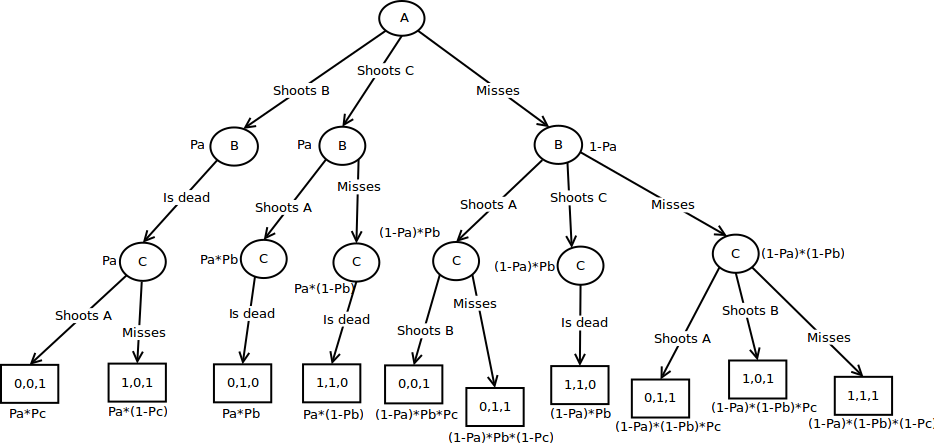
\includegraphics[scale=0.65]{SequentialTruelDiagram.png}
\end{figure}

\end{landscape}

The Diagram shows all possible actions of all players with all possible outcomes. The lowest level leaf indicates which player is still alive and with which probability - [0,0,1] indicates Player A and B being dead while Player C is alive with a probability of $p_a \times p_c$.

%%%%%%%%%%%%%%%%%%%%%%%%%%%%%%%%%%%%%%%%%%%%%%%%%%%%%%%%%%%%%%%%%%%%%%%%%
%% Bibliography start
\newpage

\bibliographystyle{unsrt}
\bibliography{bibliography}

\end{document}
